\documentclass[aspectratio=169, 10pt]{beamer}

% --- PACKAGES ---
\usepackage[utf8]{inputenc}
\usepackage{amsmath, amssymb, amsfonts}
\usepackage{graphicx}
\usepackage{booktabs}
\usepackage{colortbl}
\usepackage{array}
\usepackage{tabularx}
\usepackage{tikz}
\usetikzlibrary{positioning, calc, shapes.geometric, backgrounds, patterns, fit}
\usepackage[many]{tcolorbox}
\usepackage{fontawesome5}

% --- NORDIC COLOR PALETTE ---
\definecolor{NordicDark}{HTML}{1E293B}   % Deep Slate / Midnight
\definecolor{NordicNavy}{HTML}{0F172A}   % Dark Blue-Gray
\definecolor{NordicBlue}{HTML}{2563EB}   % Cobalt Ice Accent
\definecolor{NordicLightBlue}{HTML}{DBEAFE} % Soft Ice Tint
\definecolor{NordicTeal}{HTML}{0D9488}   % Nordic Fjord Teal
\definecolor{NordicSage}{HTML}{10B981}   % Fresh Scandinavian Pine
\definecolor{NordicBg}{HTML}{F8FAFC}     % Off-white Snow Background
\definecolor{NordicCard}{HTML}{F1F5F9}   % Soft Neutral Card
\definecolor{NordicBorder}{HTML}{E2E8F0} % Subtle Divider Border
\definecolor{NordicGray}{HTML}{64748B}   % Muted Text Gray
\definecolor{NordicText}{HTML}{0F172A}   % Primary Text Dark

% --- BEAMER THEME & SETUP ---
\mode<presentation>
\setbeamertemplate{navigation symbols}{}
\setbeamercolor{background canvas}{bg=NordicBg}
\setbeamercolor{normal text}{fg=NordicText}
\setbeamercolor{structure}{fg=NordicBlue}

% Itemize Bullet Styling
\setbeamertemplate{itemize item}{\color{NordicBlue}\small$\blacksquare$}
\setbeamertemplate{itemize subitem}{\color{NordicTeal}\scriptsize$\bullet$}
\setbeamertemplate{itemize subsubitem}{\color{NordicGray}\tiny$\bullet$}

% Frame Title Template
\setbeamertemplate{frametitle}{
  \vspace*{0.1cm}
  \begin{minipage}{\textwidth}
    {\usebeamerfont{frametitle}\color{NordicDark}\bfseries\Large\insertframetitle}\par
    \ifx\insertframesubtitle\@empty\else
      \vspace*{1pt}
      {\usebeamerfont{framesubtitle}\color{NordicGray}\small\insertframesubtitle}\par
    \fi
  \end{minipage}
  \vspace*{0.02cm}
}

% Footline Template
\setbeamertemplate{footline}{
  \ifnum\insertframenumber>1
    \begin{beamercolorbox}[wd=\paperwidth,ht=2.2ex,dp=0.8ex,leftskip=0.8cm,rightskip=0.8cm]{footline}
      \color{NordicBorder}\hrule height 0.5pt
      \vspace*{0.06cm}
      \color{NordicGray}\scriptsize
      \faGraduationCap\ \,CS 402: Distributed Systems Architecture
      \hfill
      \color{NordicGray}\scriptsize Synapse Institute of Technology
      \hfill
      \color{NordicBlue}\bfseries\insertframenumber\,/\,\inserttotalframenumber
    \end{beamercolorbox}
    \vspace*{0.04cm}
  \fi
}

% --- TCOLORBOX CUSTOM STYLES ---
\tcbuselibrary{skins, breakable}

\tcbset{
  nordiccard/.style={
    enhanced,
    colback=NordicCard,
    colframe=NordicBorder,
    boxrule=0.6pt,
    arc=3pt,
    left=5pt, right=5pt, top=3pt, bottom=3pt,
    fonttitle=\bfseries\color{NordicDark},
    coltitle=NordicDark
  },
  nordicaccent/.style={
    enhanced,
    colback=NordicLightBlue!40,
    colframe=NordicBlue,
    boxrule=0pt,
    leftrule=3.5pt,
    arc=2pt,
    left=5pt, right=5pt, top=3pt, bottom=3pt
  },
  nordictealbox/.style={
    enhanced,
    colback=NordicTeal!8,
    colframe=NordicTeal,
    boxrule=0pt,
    leftrule=3.5pt,
    arc=2pt,
    left=5pt, right=5pt, top=3pt, bottom=3pt
  }
}

\begin{document}

% ==========================================
% SLIDE 1: TITLE SLIDE
% ==========================================
\begin{frame}[plain]
  \begin{tikzpicture}[remember picture, overlay]
    % Background minimalist geo shapes
    \fill[NordicCard] (current page.north west) rectangle ($(current page.south west)+(3.8cm,0)$);
    \fill[NordicBlue] ($(current page.north west)+(3.8cm,0)$) rectangle ($(current page.south west)+(3.95cm,0)$);
    
    % Decorative soft circle in bottom right
    \fill[NordicLightBlue!30] ($(current page.south east)+(-2cm,2cm)$) circle (4cm);
    \fill[NordicTeal!10] ($(current page.south east)+(-4cm,1cm)$) circle (2.5cm);
  \end{tikzpicture}

  \vspace*{-0.2cm}
  \begin{columns}[c]
    \begin{column}{0.30\textwidth}
      \begin{center}
        {\color{NordicBlue}\Huge\faServer}\\[0.15cm]
        {\color{NordicDark}\bfseries\scriptsize LECTURE SERIES}\\[0.05cm]
        {\color{NordicGray}\tiny ADVANCED COMPUTER SCIENCE}\\[0.4cm]
        
        \tcbset{colback=white, colframe=NordicBorder, arc=3pt, boxrule=0.5pt, halign=center}
        \begin{tcolorbox}[width=0.9\linewidth]
          {\color{NordicBlue}\bfseries\tiny MODULE 04}\\[1pt]
          {\color{NordicDark}\tiny Scalable Networks}
        \end{tcolorbox}
      \end{center}
    \end{column}

    \begin{column}{0.65\textwidth}
      {\color{NordicBlue}\bfseries\tiny SYNAPSE INSTITUTE OF TECHNOLOGY}\\[0.1cm]
      {\color{NordicDark}\Large\bfseries Data-Driven Architecture \&\ Distributed Systems}\\[0.15cm]
      {\color{NordicGray}\small Patterns for Scalability, Consistency, and Resilient Storage}\\[0.25cm]
      
      \color{NordicBorder}\hrule height 0.6pt
      \vspace*{0.2cm}

      \begin{minipage}{0.48\textwidth}
        {\color{NordicGray}\tiny LECTURER}\\[1pt]
        {\color{NordicDark}\bfseries\scriptsize Dr. Erik Lindqvist}\\[1pt]
        {\color{NordicGray}\tiny Chair of Distributed Systems}
      \end{minipage}
      \begin{minipage}{0.48\textwidth}
        {\color{NordicGray}\tiny ACADEMIC TERM}\\[1pt]
        {\color{NordicDark}\bfseries\scriptsize Autumn Semester 2026}\\[1pt]
        {\color{NordicGray}\tiny Course Code: CS 402}
      \end{minipage}
    \end{column}
  \end{columns}
\end{frame}

% ==========================================
% SLIDE 2: AGENDA
% ==========================================
\begin{frame}{Lecture Agenda}{Key Topics \&\ Session Structure}
  \vspace*{-0.3cm}
  \begin{columns}[T]
    \begin{column}{0.48\textwidth}
      \begin{tcolorbox}[nordiccard, title={\color{NordicBlue}\faLayerGroup\ \,Part I: Architectural Foundations}]
        \begin{itemize}
          \item \textbf{Monolith vs. Microservices}
          \item \textbf{Fallacies of Network Computing}
          \item \textbf{CAP Theorem \&\ PACELC Trade-offs}
        \end{itemize}
      \end{tcolorbox}
      
      \vspace*{0.05cm}
      
      \begin{tcolorbox}[nordiccard, title={\color{NordicTeal}\faDatabase\ \,Part II: Storage \& Caching}]
        \begin{itemize}
          \item \textbf{Multi-Tier Data Caching (Redis)}
          \item \textbf{Write-Through vs. Write-Back}
          \item \textbf{Database Sharding Strategies}
        \end{itemize}
      \end{tcolorbox}
    \end{column}

    \begin{column}{0.48\textwidth}
      \begin{tcolorbox}[nordiccard, title={\color{NordicBlue}\faCloud\ \,Part III: Production Case Study}]
        \begin{itemize}
          \item \textbf{Meridian Platform Traffic Spikes}
          \item \textbf{1.2M Concurrent Connections}
          \item \textbf{Empirical Latency Metrics}
        \end{itemize}
      \end{tcolorbox}
      
      \vspace*{0.05cm}
      \begin{tcolorbox}[nordiccard, title={\color{NordicTeal}\faLock\ \,Part IV: Resiliency Engineering}]
        \begin{itemize}
          \item \textbf{Circuit Breakers \&\ Backoff}
          \item \textbf{Distributed Consensus (Raft Engine)}
          \item \textbf{Summary \&\ System Checklist}
        \end{itemize}
      \end{tcolorbox}
    \end{column}
  \end{columns}
\end{frame}

% ==========================================
% SLIDE 3: SECTION DIVIDER 1
% ==========================================
\begin{frame}[plain]
  \begin{tikzpicture}[remember picture, overlay]
    \fill[NordicDark] (current page.north west) rectangle (current page.south east);
    \fill[NordicTeal!30] ($(current page.north east)+(-3cm,0)$) -- (current page.north east) -- (current page.south east) -- ($(current page.south east)+(-6cm,0)$) -- cycle;
    \fill[NordicBlue] ($(current page.south west)+(0,2cm)$) rectangle ($(current page.south east)+(0,2.15cm)$);
  \end{tikzpicture}
  
  \vspace*{1.2cm}
  \begin{center}
    {\color{NordicTeal}\bfseries\small MODULE 01}\\[0.3cm]
    {\color{white}\Huge\bfseries Architectural Foundations}\\[0.3cm]
    {\color{NordicBorder}\small Deconstructing Distributed Complexity \&\ Consistency Guarantees}
  \end{center}
\end{frame}

% ==========================================
% SLIDE 4: MONOLITH VS MICROSERVICES
% ==========================================
\begin{frame}{System Paradigms}{Comparing Monolithic and Distributed Microservices}
  \vspace*{-0.35cm}
  \begin{columns}[T]
    \begin{column}{0.48\textwidth}
      \begin{tcolorbox}[nordicaccent]
        {\color{NordicDark}\bfseries Monolithic Architecture}\\[0.05cm]
        {\color{NordicGray}\scriptsize Single unified codebase and deployment artifact.}
        \vspace*{0.05cm}
        \begin{itemize}
          \item \textbf{Memory Access:} In-process calls ($<1\,\mu\text{s}$).
          \item \textbf{Transactions:} ACID via single RDBMS.
          \item \textbf{Scaling:} Vertical scale-up (CPU/RAM).
          \item \textbf{Deployment:} Tightly coupled releases.
        \end{itemize}
      \end{tcolorbox}
    \end{column}

    \begin{column}{0.48\textwidth}
      \begin{tcolorbox}[nordictealbox]
        {\color{NordicDark}\bfseries Distributed Microservices}\\[0.05cm]
        {\color{NordicGray}\scriptsize Decoupled services over network RPC.}
        \vspace*{0.05cm}
        \begin{itemize}
          \item \textbf{Network RPC:} Remote API calls ($5\text{--}50\,\text{ms}$).
          \item \textbf{Transactions:} BASE / Eventual consistency.
          \item \textbf{Scaling:} Horizontal scale-out (elastic).
          \item \textbf{Deployment:} Independent CI/CD pipelines.
        \end{itemize}
      \end{tcolorbox}
    \end{column}
  \end{columns}

  \vspace*{0.05cm}
  \begin{tcolorbox}[nordiccard]
    {\color{NordicDark}\bfseries Key Insight:} Transitioning to microservices trades \textbf{code complexity} for \textbf{operational complexity}. Network topology becomes a primary design constraint.
  \end{tcolorbox}
\end{frame}

% ==========================================
% SLIDE 5: CAP THEOREM & PACELC
% ==========================================
\begin{frame}{The CAP Theorem \&\ PACELC Framework}{Fundamental Trade-offs in Distributed Data}
  \vspace*{-0.3cm}
  \begin{columns}[T]
    \begin{column}{0.55\textwidth}
      \begin{itemize}
        \item \textbf{Consistency (C):} Every read receives the most recent write or an error.
        \item \textbf{Availability (A):} Every non-failing node returns a non-error response.
        \item \textbf{Partition Tolerance (P):} System functions despite network dropouts.
      \end{itemize}

      \vspace*{0.1cm}
      \begin{tcolorbox}[nordicaccent]
        {\color{NordicBlue}\bfseries The PACELC Extension:}\\[2pt]
        {\scriptsize \textbf{If Partition (P):} Choose Availability (A) vs. Consistency (C).\\[1pt]
        \textbf{Else (E):} Choose Latency (L) vs. Consistency (C).}
      \end{tcolorbox}
    \end{column}

    \begin{column}{0.42\textwidth}
      \begin{center}
        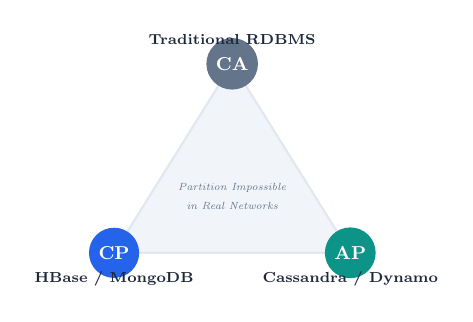
\begin{tikzpicture}[scale=0.75, every node/.style={transform shape}]
          % CAP Triangle
          \draw[thick, NordicBorder, fill=NordicCard] (0,0) -- (4,0) -- (2,3.2) -- cycle;
          
          % Nodes
          \node[circle, fill=NordicBlue, text=white, font=\bfseries\small, inner sep=3pt] at (0,0) {CP};
          \node[circle, fill=NordicTeal, text=white, font=\bfseries\small, inner sep=3pt] at (4,0) {AP};
          \node[circle, fill=NordicGray, text=white, font=\bfseries\small, inner sep=3pt] at (2,3.2) {CA};
          
          % Labels
          \node[below, font=\scriptsize\bfseries, color=NordicDark] at (0,-0.2) {HBase / MongoDB};
          \node[below, font=\scriptsize\bfseries, color=NordicDark] at (4,-0.2) {Cassandra / Dynamo};
          \node[above, font=\scriptsize\bfseries, color=NordicDark] at (2,3.4) {Traditional RDBMS};
          
          \node[font=\tiny\itshape, color=NordicGray] at (2,1.1) {Partition Impossible};
          \node[font=\tiny\itshape, color=NordicGray] at (2,0.8) {in Real Networks};
        \end{tikzpicture}
      \end{center}
    \end{column}
  \end{columns}
\end{frame}

% ==========================================
% SLIDE 6: FALLACIES OF DISTRIBUTED COMPUTING
% ==========================================
\begin{frame}{Fallacies of Distributed Computing}{Common Architectural Pitfalls in Production}
  \vspace*{-0.3cm}
  \begin{columns}[T]
    \begin{column}{0.48\textwidth}
      \begin{tcolorbox}[nordiccard, title={\color{NordicBlue}\faExclamationTriangle\ \,Network Assumptions}]
        \begin{enumerate}
          \item \textbf{Network is reliable:} Packets drop, routers fail.
          \item \textbf{Latency is zero:} Round-trips dominate execution.
          \item \textbf{Bandwidth is infinite:} Saturation degrades nodes.
        \end{enumerate}
      \end{tcolorbox}
    \end{column}

    \begin{column}{0.48\textwidth}
      \begin{tcolorbox}[nordiccard, title={\color{NordicTeal}\faNetworkWired\ \,Topology Assumptions}]
        \begin{enumerate}\setcounter{enumii}{3}
          \item \textbf{Network is secure:} Internal traffic needs auth.
          \item \textbf{Topology is static:} Containers scale dynamically.
          \item \textbf{Transport cost is zero:} Serialization takes CPU.
        \end{enumerate}
      \end{tcolorbox}
    \end{column}
  \end{columns}

  \vspace*{0.1cm}
  \begin{tcolorbox}[nordictealbox]
    {\color{NordicDark}\bfseries Architectural Rule:} Always design for asynchronous failure. Assume network requests will fail, timeout, or arrive out of order.
  \end{tcolorbox}
\end{frame}

% ==========================================
% SLIDE 7: SECTION DIVIDER 2
% ==========================================
\begin{frame}[plain]
  \begin{tikzpicture}[remember picture, overlay]
    \fill[NordicDark] (current page.north west) rectangle (current page.south east);
    \fill[NordicBlue!25] ($(current page.north west)+(0,0)$) -- ($(current page.north west)+(6cm,0)$) -- ($(current page.south west)+(3cm,0)$) -- (current page.south west) -- cycle;
    \fill[NordicTeal] ($(current page.south west)+(0,2cm)$) rectangle ($(current page.south east)+(0,2.15cm)$);
  \end{tikzpicture}
  
  \vspace*{1.2cm}
  \begin{center}
    {\color{NordicBlue}\bfseries\small MODULE 02}\\[0.3cm]
    {\color{white}\Huge\bfseries Storage Systems \&\ Caching Strategies}\\[0.3cm]
    {\color{NordicBorder}\small Optimizing Memory Hierarchies and Database Invalidation}
  \end{center}
\end{frame}

% ==========================================
% SLIDE 8: TIKZ ARCHITECTURE DIAGRAM
% ==========================================
\begin{frame}{Multi-Tier Storage Architecture}{Data Flow Through In-Memory Caching and Persistent Storage}
  \vspace*{-0.3cm}
  \begin{center}
    \begin{tikzpicture}[node distance=1.3cm, auto, >=stealth, scale=0.80, every node/.style={transform shape}]
      % Style definitions
      \tikzstyle{client} = [rectangle, draw=NordicBlue, fill=NordicLightBlue!50, thick, minimum width=2.0cm, minimum height=0.85cm, rounded corners=4pt, align=center, font=\bfseries\small]
      \tikzstyle{gateway} = [rectangle, draw=NordicDark, fill=NordicCard, thick, minimum width=2.2cm, minimum height=0.85cm, rounded corners=4pt, align=center, font=\bfseries\small]
      \tikzstyle{cache} = [rectangle, draw=NordicTeal, fill=NordicTeal!15, thick, minimum width=2.4cm, minimum height=0.85cm, rounded corners=4pt, align=center, font=\bfseries\small]
      \tikzstyle{db} = [cylinder, draw=NordicDark, fill=NordicDark!10, thick, minimum width=1.8cm, minimum height=1.0cm, cylinder end fill=NordicDark!20, shape border rotate=90, align=center, font=\bfseries\small]

      % Nodes
      \node[client] (user) {\faUser\ Client App};
      \node[gateway, right=1.1cm of user] (api) {\faRoute\ API Gateway\\(Nexa Proxy)};
      \node[cache, right=1.1cm of api] (redis) {\faMemory\ Redis Cache\\(In-Memory)};
      \node[db, right=1.3cm of redis] (db) {\faDatabase\ PostgreSQL\\(Primary DB)};

      % Connections
      \draw[->, very thick, NordicDark] (user) -- node[above, font=\tiny\bfseries] {HTTPS Req} (api);
      
      \draw[->, very thick, NordicBlue] (api) -- node[above, font=\tiny\bfseries] {1. Check Cache} (redis);
      \draw[->, dashed, thick, NordicTeal] (redis) edge[bend left=25] node[below, font=\tiny\bfseries] {Cache Hit ($<2\,\text{ms}$)} (api);
      
      \draw[->, very thick, NordicDark] (redis) -- node[above, font=\tiny\bfseries] {2. Cache Miss} (db);
      \draw[->, dashed, thick, NordicGray] (db) edge[bend left=30] node[below, font=\tiny\bfseries] {3. Return Data} (redis);

      % Background Container Box using fit library
      \begin{scope}[on background layer]
        \node[draw=NordicBorder, fill=NordicBg, dashed, rounded corners=6pt, inner sep=6pt, fit=(api) (redis) (db)] {};
      \end{scope}
    \end{tikzpicture}
  \end{center}

  \vspace*{-0.15cm}
  \begin{columns}[T]
    \begin{column}{0.48\textwidth}
      \begin{tcolorbox}[nordicaccent]
        {\color{NordicBlue}\bfseries L1 In-Memory Cache Tier}\\[2pt]
        {\scriptsize Delivers sub-millisecond read performance for hot data keys (95\% hit target rate).}
      \end{tcolorbox}
    \end{column}
    \begin{column}{0.48\textwidth}
      \begin{tcolorbox}[nordictealbox]
        {\color{NordicTeal}\bfseries Persistent Storage Tier}\\[2pt]
        {\scriptsize Ensures ACID durability for critical state with write-ahead logging (WAL).}
      \end{tcolorbox}
    \end{column}
  \end{columns}
\end{frame}

% ==========================================
% SLIDE 9: CACHE INVALIDATION TABLE
% ==========================================
\begin{frame}{Cache Consistency Patterns}{Comparative Analysis of Invalidation Strategies}
  \vspace*{-0.3cm}
  \begin{center}
    \fontsize{8pt}{9.5pt}\selectfont
    \rowcolors{2}{NordicCard!50}{white}
    \begin{tabularx}{\textwidth}{l X X X}
      \toprule
      \rowcolor{NordicDark}
      \color{white}\textbf{Pattern} & \color{white}\textbf{Write Flow} & \color{white}\textbf{Latency Profile} & \color{white}\textbf{Primary Use Case} \\
      \midrule
      \textbf{Cache-Aside} & App writes to DB; invalidates key. & Read penalty on miss; low write latency. & General web apps, dynamic feeds. \\
      \textbf{Write-Through} & App writes to Cache; Cache writes DB synchronously. & Higher write latency; guaranteed consistency. & Financial ledgers, transactions. \\
      \textbf{Write-Back} & App writes to Cache; async write to DB. & Lowest write latency; risk of data loss. & Analytics \&\ telemetry logs. \\
      \textbf{Refresh-Ahead} & Cache auto-refreshes hot keys prior to TTL. & Optimal read latency; complex setup. & High-traffic static catalogs. \\
      \bottomrule
    \end{tabularx}
  \end{center}

  \vspace*{0.05cm}
  \begin{tcolorbox}[nordiccard]
    {\color{NordicDark}\bfseries Phil Karlton's Adage:} \textit{"There are only two hard things in Computer Science: cache invalidation and naming things."}
  \end{tcolorbox}
\end{frame}

% ==========================================
% SLIDE 10: SECTION DIVIDER 3
% ==========================================
\begin{frame}[plain]
  \begin{tikzpicture}[remember picture, overlay]
    \fill[NordicDark] (current page.north west) rectangle (current page.south east);
    \fill[NordicSage!25] ($(current page.north east)+(-5cm,0)$) -- (current page.north east) -- (current page.south east) -- ($(current page.south east)+(-2cm,0)$) -- cycle;
    \fill[NordicSage] ($(current page.south west)+(0,2cm)$) rectangle ($(current page.south east)+(0,2.15cm)$);
  \end{tikzpicture}
  
  \vspace*{1.2cm}
  \begin{center}
    {\color{NordicSage}\bfseries\small MODULE 03}\\[0.3cm]
    {\color{white}\Huge\bfseries Production Case Study: Meridian Cloud}\\[0.3cm]
    {\color{NordicBorder}\small Real-World High-Concurrency Load Handling \&\ Scaling Metrics}
  \end{center}
\end{frame}

% ==========================================
% SLIDE 11: MERIDIAN CASE STUDY
% ==========================================
\begin{frame}{Case Study: Meridian Cloud Platform}{Handling Flash Traffic Spikes during Global Events}
  \vspace*{-0.3cm}
  \begin{columns}[T]
    \begin{column}{0.48\textwidth}
      \begin{tcolorbox}[nordiccard, title={\color{NordicDark}\faSearch\ \,The Challenge}]
        \begin{itemize}
          \item Peak load burst: \textbf{1.2M req/sec} during event.
          \item Primary DB CPU saturated at \textbf{99.4\%}.
          \item Cascading failures across microservices.
        \end{itemize}
      \end{tcolorbox}
    \end{column}

    \begin{column}{0.48\textwidth}
      \begin{tcolorbox}[nordicaccent, title={\color{NordicBlue}\faTools\ \,The Engineering Solution}]
        \begin{itemize}
          \item Implemented \textbf{Rate Limiting} via Redis.
          \item Deployed \textbf{Consistent Hashing} on storage.
          \item Enforced queueing via \textbf{Vertex Message Bus}.
        \end{itemize}
      \end{tcolorbox}
    \end{column}
  \end{columns}

  \vspace*{0.1cm}
  \begin{tcolorbox}[nordictealbox]
    {\color{NordicTeal}\bfseries Outcome:} System stabilized with zero database crashes and average response time reduced from \textbf{4,200\,ms} to \textbf{38\,ms} at 99th percentile.
  \end{tcolorbox}
\end{frame}

% ==========================================
% SLIDE 12: EMPIRICAL PERFORMANCE METRICS
% ==========================================
\begin{frame}{Empirical System Metrics}{Post-Optimization Performance Benchmarks at Meridian}
  \vspace*{-0.3cm}
  \begin{columns}[T]
    \begin{column}{0.31\textwidth}
      \begin{tcolorbox}[nordiccard]
        \begin{center}
          {\color{NordicBlue}\Large\bfseries -98.2\%}\\[0.05cm]
          {\color{NordicDark}\bfseries\small Latency Reduction}\\[0.1cm]
          {\color{NordicGray}\tiny P99 latency dropped from 4.2s to 38ms post-caching.}
        \end{center}
      \end{tcolorbox}
    \end{column}

    \begin{column}{0.31\textwidth}
      \begin{tcolorbox}[nordiccard]
        \begin{center}
          {\color{NordicTeal}\Large\bfseries 99.999\%}\\[0.05cm]
          {\color{NordicDark}\bfseries\small High Availability}\\[0.1cm]
          {\color{NordicGray}\tiny Five-nines uptime maintained across 90-day window.}
        \end{center}
      \end{tcolorbox}
    \end{column}

    \begin{column}{0.31\textwidth}
      \begin{tcolorbox}[nordiccard]
        \begin{center}
          {\color{NordicNavy}\Large\bfseries 4.5x}\\[0.05cm]
          {\color{NordicDark}\bfseries\small Throughput Gain}\\[0.1cm]
          {\color{NordicGray}\tiny Sustained requests/sec increased without added hardware.}
        \end{center}
      \end{tcolorbox}
    \end{column}
  \end{columns}

  \vspace*{0.15cm}
  \begin{tcolorbox}[nordicaccent]
    {\color{NordicDark}\bfseries Key Observation:} Caching and queueing decoupled compute spikes from persistent storage, converting catastrophic failures into controlled queue latency.
  \end{tcolorbox}
\end{frame}

% ==========================================
% SLIDE 13: SECTION DIVIDER 4
% ==========================================
\begin{frame}[plain]
  \begin{tikzpicture}[remember picture, overlay]
    \fill[NordicDark] (current page.north west) rectangle (current page.south east);
    \fill[NordicBlue!40] ($(current page.south west)+(0,0)$) -- ($(current page.south west)+(8cm,0)$) -- ($(current page.north west)+(4cm,0)$) -- (current page.north west) -- cycle;
    \fill[NordicTeal] ($(current page.south west)+(0,2cm)$) rectangle ($(current page.south east)+(0,2.15cm)$);
  \end{tikzpicture}
  
  \vspace*{1.2cm}
  \begin{center}
    {\color{NordicLightBlue}\bfseries\small MODULE 04}\\[0.3cm]
    {\color{white}\Huge\bfseries Resiliency Engineering \& Summary}\\[0.3cm]
    {\color{NordicBorder}\small Fault Isolation, Graceful Degradation, and Architectural Guidelines}
  \end{center}
\end{frame}

% ==========================================
% SLIDE 14: CIRCUIT BREAKER PATTERN
% ==========================================
\begin{frame}{Circuit Breaker Pattern}{Preventing Cascading System Failures}
  \vspace*{-0.3cm}
  \begin{columns}[T]
    \begin{column}{0.55\textwidth}
      \begin{tcolorbox}[nordiccard, title={\color{NordicDark}\faToggleOn\ \,State Machine Lifecycle}]
        \begin{itemize}
          \item \textbf{Closed State:} Normal operations. Traffic flows freely to downstream service.
          \item \textbf{Open State:} Error threshold exceeded ($>15\%$). Calls fail fast immediately.
          \item \textbf{Half-Open State:} Trial period. Probes service with test traffic.
        \end{itemize}
      \end{tcolorbox}
    \end{column}

    \begin{column}{0.42\textwidth}
      \begin{tcolorbox}[nordictealbox, title={\color{NordicTeal}\faCode\ \,Implementation Rule}]
        {\scriptsize
        \texttt{if (errors > threshold) \{\\
        \ \ \ openBreaker();\\
        \ \ \ return fallbackData();\\
        \} else \{\\
        \ \ \ executeServiceCall();\\
        \}}
        }
      \end{tcolorbox}
      
      \vspace*{0.05cm}
      \begin{tcolorbox}[nordicaccent]
        {\color{NordicBlue}\bfseries Combined Pattern:}\\[2pt]
        {\scriptsize Pair Circuit Breakers with \textbf{Exponential Backoff} and randomized \textbf{Jitter}.}
      \end{tcolorbox}
    \end{column}
  \end{columns}
\end{frame}

% ==========================================
% SLIDE 15: ARCHITECTURAL CHECKLIST
% ==========================================
\begin{frame}{Architectural Checklist}{Design Principles for Distributed Systems}
  \vspace*{-0.3cm}
  \begin{columns}[T]
    \begin{column}{0.48\textwidth}
      \begin{tcolorbox}[nordiccard, title={\color{NordicBlue}\faCheckSquare\ \,System Design Musts}]
        \begin{itemize}
          \item \textbf{Idempotency:} Ensure API writes can be retried with UUID.
          \item \textbf{Stateless Services:} Offload session state to Redis.
          \item \textbf{Graceful Degradation:} Serve cached data if primary fails.
        \end{itemize}
      \end{tcolorbox}
    \end{column}

    \begin{column}{0.48\textwidth}
      \begin{tcolorbox}[nordiccard, title={\color{NordicTeal}\faExclamationCircle\ \,Operational Anti-Patterns}]
        \begin{itemize}
          \item \textbf{Distributed Transactions:} Avoid 2PC across microservices.
          \item \textbf{Hardcoded Endpoints:} Utilize dynamic Discovery (K8s).
          \item \textbf{Shared Databases:} Never allow services to share raw DB.
        \end{itemize}
      \end{tcolorbox}
    \end{column}
  \end{columns}

  \vspace*{0.1cm}
  \begin{tcolorbox}[nordictealbox]
    {\color{NordicDark}\bfseries Golden Rule:} Prioritize simplicity. Distributed systems are inherently complex; avoid adding unnecessary distribution unless required by scale.
  \end{tcolorbox}
\end{frame}

% ==========================================
% SLIDE 16: CLOSING & Q&A
% ==========================================
\begin{frame}[plain]
  \begin{tikzpicture}[remember picture, overlay]
    \fill[NordicDark] (current page.north west) rectangle (current page.south east);
    \fill[NordicLightBlue!20] ($(current page.north west)+(0,-2cm)$) circle (5cm);
    \fill[NordicTeal!20] ($(current page.south east)+(-1cm,1cm)$) circle (4cm);
    \fill[NordicBlue] ($(current page.south west)+(0,1cm)$) rectangle ($(current page.south east)+(0,1.15cm)$);
  \end{tikzpicture}

  \vspace*{1.0cm}
  \begin{center}
    {\color{NordicTeal}\Huge\bfseries Thank You!}\\[0.3cm]
    {\color{white}\Large Questions \&\ Discussion}\\[0.4cm]
    
    \begin{tcolorbox}[width=0.75\textwidth, colback=white!10, colframe=NordicBorder!30, arc=4pt, halign=center]
      {\color{white}\small\faEnvelope\ \,erik.lindqvist@synapse.edu \qquad \faGlobe\ \,https://synapse.edu/cs402}\\[0.15cm]
      {\color{NordicBorder}\scriptsize Office Hours: Tuesdays 14:00--16:00 | Campus Building 04, Room 302}
    \end{tcolorbox}
  \end{center}
\end{frame}

\end{document}
